\section{\scshape Okno Parzena}

\begin{frame}{Okno Parzena}
\begin{itemize}
	\item Technika interpolacji danych.
	\item Szacuje warto"sć funkcji gęsto"sci prawdopodobieństwa dla danej próbki.
	\item Wykorzystuje okno o zadanym rozmiarze.

\end{itemize}
\end{frame}

\note{Mając daną losową próbkę, okno Parzena pozwala oszacować warto"sć funkcji gęsto"sci prawdopodobieństwa. \\
Każda próbka mieszcząca się w oknie wpływa na wspomniane oszacowanie. \\
Technikę wykorzystuje się również do klasyfikacji.
}

\begin{frame}{Sposób szacowania}
\begin{itemize}
	\item Ustawienie okna na próbce $x$.
	\item Badanie obserwacji $x_i$ mieszczących się w oknie.
	\item Obliczanie warto"sci funkcji gęsto"sci P(x) ze wzoru:
	\begin{equation}
	P(x) = \frac{1}{n}\sum_{i=1}^n\frac{1}{h_n^d}K(\frac{x-x_i}{h_n})
	\end{equation}
\end{itemize}
\end{frame}

\note{$n$ okre"sla liczbę obserwacji, $h$ to rozmiar okna. \\ $K(\frac{x-x_i}{h_n})$ definiuje funkcję okna. Jej całka równa się $1$. Dla obserwacji znajdujących coraz bliżej próbki $x$ funkcja zwraca większe lub równe warto"sci. \\
Jednym z przykładów funkcji okna jest funkcja Gaussa.}

\begin{frame}{Przykładowe użycie}
	
\begin{center}
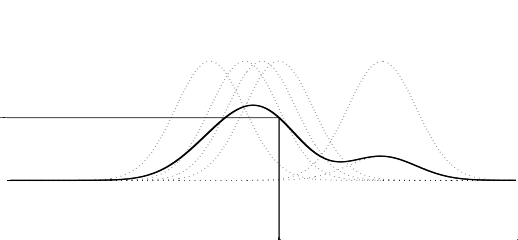
\includegraphics[keepaspectratio=true, scale=0.55]{parzen_small}
\end{center}
	
	
\begin{equation}
	P(x) = \frac{1}{n}\sum_{i=1}^n\frac{1}{\sqrt{2\pi\sigma}}e^{-\frac{(x-x_i)^2}{2\sigma^2}}
\end{equation}
\end{frame}

\note{Jako funkcji okna użyto funkcji Gaussa. \\
Zbiór obserwacji składa się z $5$ punktów. \\
Każdy punkt ma wkład w oszacowanie. Linie kropkowane przedstawiają funkcje Gaussowskie wokół punktów zbioru obserwacji.}


\begin{frame}{Zastosowania}
\begin{itemize}
	\item Rozpoznawanie wzroców.
	\item Klasyfikacja.
	\item Analiza i odtwarzanie obrazów.

\end{itemize}
\end{frame}



	
